\documentclass[a4paper]{report}
\pagestyle{headings}
\usepackage{hyperref}
\usepackage{listings}
\usepackage{graphicx}
\usepackage{subfiles}
\usepackage{multirow}
\usepackage[table,xcdraw]{xcolor}
\lstset{numbers=right}
\lstset{breaklines}
\title{Lab Report for Software Engineering course \newline
 Lab 6: Demand Documentation}
\author{Wang, Chen\qquad Liu, Jiaxing\qquad Huang, Jiani\qquad Tang, Xinyue \\
16307110064\qquad17302010049\qquad 17302010063\qquad 16307110476 \\
School of Software\\
Fudan University
}
\date{\today}
\bibliographystyle{plain}
\begin{document}
\maketitle

\tableofcontents
\chapter{Revision History of the demand documentation}

\begin{tabular}{|c|c|c|l|}
\hline 
Modifier&Modify Time&Approver&Modified Chapter\\
\hline  
Wang, Chen&Jun 9, 2019&All&Initial outline of the documentation\\
\hline 
Wang, Chen&Jun 10, 2019&All&Detailed outline of the documentation\\
\hline 
Huang, Jiani&Jun 13, 2019&All&Initial refined requirements\\
\hline 
Huang, Jiani&Jun 14, 2019&All&Revised refined requirements\\
\hline 
Huang, Jiani&Jun 14, 2019&All&Add the four diagrams\\
\hline 
Huang, Jiani&Jun 19, 2019&All&Refined Function Requirements\\
\hline 
Wang, Chen&Jun 19, 2019&All&Add the demand interview outline\\
\hline
Huang, Jiani&Jun 19, 2019&All&Add the diagrams\\
\hline
Huang, Jiani&Jun 19, 2019&All&Add the use case diagram\\
\hline
Wang, Chen&Jun 19, 2019&All&Rename the pdf figure file name\\
\hline
Huang, Jiani&Jun 19, 2019&All&Revise some expressions\\
\hline
Wang, Chen&Jun 19, 2019&All&Replace the jpg figure with the pdf versions\\
\hline
Wang, Chen&Jun 20, 2019&All&Add the background information section\\
\hline
Wang, Chen&Jun 20, 2019&All&Add the feature overview section\\
\hline
Wang, Chen&Jun 20, 2019&All&Add the module division, user characteristics \\
& & & section\\
\hline
Huang, Jiani&Jun 20, 2019&All&Revise some words\\
\hline
Wang, Chen&Jun 20, 2019&All&Add the system configuration parts\\
\hline
Huang, Jiani&Jun 20, 2019&All&Add performance needs part\\
\hline
Huang, Jiani&Jun 20, 2019&All&Revise some expressions\\
\hline
Wang, Chen&Jun 20, 2019&All&Add the client side system configuration part\\
\hline
Wang, Chen&Jun 21, 2019&All&Removed temp files\\
\hline
Wang, Chen&Jun 21, 2019&All&Add the server side and client side price \\
& & &description\\
\hline
Wang, Chen&Jun 22, 2019&All&Add the terms and conditions\\
\hline
Wang, Chen&Jun 22, 2019&All&Add the functional requirements\\
\hline
Wang, Chen&Jun 22, 2019&All&Add the constraints part\\
\hline
Huang, Jiani&Jun 22, 2019&All&Revise some expressions\\
\hline
Huang, Jiani&Jun 22, 2019&All&Correct the file name\\
\hline
Wang, Chen&Jun 22, 2019&All&Add part of the documentation history part\\
\hline
Wang, Chen&Jun 22, 2019&All&Add the documentation history part\\
\hline
\end{tabular}

\chapter{Project Outline}
\section{Background information of the project}
Now some customers come here to make a request to Star Dad, and hope that the development team can develop a beverage online sales system according to the needs of customers. Now you need to carry out the basic arrangement and rational understanding of the customer's needs (which are specified more clearly in the next section), communicate with the customer, conduct line analysis and refinement, and guide the development of the development team.
\par
\subsection{General demands of the project}
There are two specific restrictions or conditions about the project:
\begin{enumerate}
\item
Number of users: 1000 people / day
\item
Budget: 1 million yuan

\end{enumerate}

\section{Overview of the features of the project}
\subsection{Beverage Store}
The beverage store should have the following functions:
\begin{enumerate}
\item
Drink support: The system can support a variety of drinks from the beverage store;
\item Ingredient support: The system can support the diverse ingredients offered by the beverage store;
\item
Cup support: The system can support the variety of cups offered by the beverage store;
\item 
Preferential support: The system can support the various discounts offered by the beverage store. Currently, the discounts offered by the beverage store are as follows (these offers have certain superposition and mutual exclusion):
\begin{itemize}
\item
20\% off 2 cups of espresso
\item 
Tea buy 3 get 1 free
\item
Cappuccino 2nd Cup Half Price
\item
All items 30 yuan deduction over 100 yuan
\item 50\% off on Nov 11th
\item
15\% off for tea and coffee
\end{itemize}
\item Language support: The system can support the switching of different languages in different regions of the beverage store;
\item
Currency support: The system can support the conversion of different currencies in different regions of the beverage store;
\item
Pricing support: The system is priced according to the regulations of the beverage store.
\end{enumerate}
\par
General requirements: This system should support the beverages offered and launched by the beverage store, a variety of ingredients, these drinks have different cup types, of course, in order to sell, the system also needs to support a variety of preferential strategies launched by the beverage store, while In order to develop internationally, the system must support switching between different languages and currency conversion. Finally, the pricing of all goods must be strictly in accordance with the regulations of the beverage store.
\subsection{Salesperson}
The salesperson should have the following functions:
\begin{enumerate}
\item
Registration: The salesperson can register in the system with a valid account password;
\item
Login: The salesperson can log in using the account number and password to ensure the daily operation of the salesperson;
\item
Matching: The salesperson can use the system with different drinks when they have permission;
\item
Description: The salesperson can use the system to obtain a description of the different beverages when they have permission;
\item
Valuation: The salesperson can use the system to place orders when they have permission. After the order is placed, the price of different beverages can be calculated. The price of the beverage depends on the base price of the beverage, the price of the cup of the beverage, the price of the additional ingredients, and also consider the number of drinks. And a variety of preferential strategies.
\end{enumerate}
\par
General requirements: This system must support the salesperson to perform daily operations after obtaining the permission, including registration, registration, beverage matching, description acquisition and order placement. These daily operations must comply with the company's legal requirements. In addition, the system also needs to provide according to company regulations. Pricing function, these operations are convenient for the day-to-day operation of the salesperson.
\subsection{Development and operation personnel}
The development and operation personnel should have the following functions:
\begin{enumerate}
\item
Background maintenance: Maintenance personnel can configure and maintain various support such as drinks, ingredients, cups, offers, language, currency, pricing, etc. in the background according to company regulations;
\item
Log information: The maintenance personnel need the log information provided by the system during maintenance.
\item
Support the use of a large number of stores concurrently 
\item 
The system should be stable for a long time
\end{enumerate}
General requirements: Development and operation and maintenance personnel can perform system background maintenance according to company regulations, and provide standardized log information during system operation.
\subsection{Beverage shop customer}
The beverage shop customer should have the following functions:
\begin{enumerate}
\item
Matching: The order can be matched by the salesperson;
\item
Pricing: You can see the price of the order;
\item
Offer: Customers want the bigger the better, the better!
\item
Description: You can see a description of the different beverages, a detailed description of the beverage price, and a specific description of the specifications used.
\end{enumerate}
\par
General requirements: The customer mainly performs system operation through the salesperson. The customer cares that the system can match the beverage that he wants, and at the same time needs to see the correct price and specific description. Of course, the customer wants the bigger the better.
\section{Module division of the project}
According to the demands of the project, the project can be divided into the following divisions:
the account services division, order controller division, the beverage repository implementation division and the utility tools division.
\par
The detailed description of the divisions will be discussed in the consequent chapters.
\section{User characteristics of the project}
There are three different users having relationship with this project.
\subsection{Beverage shop customers}
The beverage shop customers are the customers coming to the beverage shop and wish to buy beverage.
\subsection{Salesperson}
The salesperson are the workers in the beverage shop who help the customers place orders, charge the customers and provide beverages to the customers.
\subsection{Development and operation personnel}
The development and operation personnel are the developers of the system who are in charge of the future maintenance of the system. They will read the log info, organize databases and modify the application in response of the future demand changes.
\section{Run time environment}
There is no obvious runtime environment restriction of the application both in the back end and in the front end.
\par
After analysis of the market, the needs and demands, and the performance of the application, we have decided to use the following runtime environment as our production. 
\subsection{Server side runtime environment}
After thorough research about the server providers, we have decided to adopt the DELL Workstation as the server to proved service. As have stated above, there are about 1,000 customers coming to a store a day and there are 200 stores in total. However, what the distribution of customer flow over time is not given and according to the description from the teaching assistants, we can see the statistics above as the average customer flow to the store. In this way, every hour there might be 200,000 order requests, indicating that the server should handle at least 50 requests a second. We have found that the Dell OptiPlex 7050 with 3.6GHz Core i7-7700 CPU meet these demands well, whose 8 cores and 8MB cache will make request handling rapidly.
\par
The price for the DELL OptiPlex 7050 with the specification below will be about \$700  and it is well within our budgets. 
\subsubsection{SYSTEM INFORMATION}
Running Ubuntu Linux, the Ubuntu 18.04 (bionic) release.
\begin{itemize}
\item GNOME: 3.28.2 (Ubuntu)
\item Kernel version: 4.15.0-36-generic (\#39-Ubuntu SMP Mon Sep 24 16:19:09 UTC 2018)
\item GCC: 7 (x86\_64-linux-gnu)
\item Xorg: unknown
\item Hostname: wangchen-OptiPlex-7050-China-HDD-Protection
\item	Uptime: 0 days 0 h 12 min
\end{itemize}
\subsubsection{CPU INFORMATION}
\begin{itemize}
\item GenuineIntel, Intel(R) Core(TM) i7-7700 CPU @ 3.60GHz
\item Number of CPUs: 8
\item CPU clock currently at 799.996 MHz with 8192 KB cache
\item Numbering: family(6) model(158) stepping(9)
\item	Bogomips: 7200.00
\end{itemize}
\subsubsection{MEMORY INFORMATION}
\begin{itemize}
\item Total memory: 7854 MB
\item Total swap: 2047 MB
\end{itemize}
\subsubsection{STORAGE INFORMATION}
\begin{itemize}
\item SCSI device -  scsi0 \begin{itemize}
\item Vendor:  ATA
\item Model:  ST1000DM003-1SB1 
\end{itemize}
\end{itemize}
\subsubsection{HARDWARE INFORMATION}
\begin{itemize}
\item MOTHERBOARD
\begin{itemize} 
\item Host bridge
\begin{itemize}
\item Intel Corporation Intel Kaby Lake Host Bridge (rev 05)
\item Subsystem: Dell Intel Kaby Lake Host Bridge
\end{itemize}
\item
PCI bridge(s)
\begin{itemize}
\item Intel Corporation 200 Series PCH PCI Express Root Port \#4 (rev f0) (prog-if 00 [Normal decode])
\item Texas Instruments XIO2001 PCI Express-to-PCI Bridge (prog-if 00 [Normal decode])
\end{itemize}
\item ISA bridge
\begin{itemize}
\item Intel Corporation 200 Series PCH LPC Controller (Q270)
\item Subsystem: Dell 200 Series PCH LPC Controller (Q270)
\end{itemize}
\end{itemize}
\item GRAPHIC CARD
\begin{itemize}
\item VGA controller
\begin{itemize}
\item Intel Corporation HD Graphics 630 (rev 04) (prog-if 00 [VGA controller])
\item Subsystem: Dell HD Graphics 630
\end{itemize}
\end{itemize}
	
\item SOUND CARD
\begin{itemize}
\item Multimedia controller
\begin{itemize} 
\item Intel Corporation 200 Series PCH HD Audio
\item Subsystem: Dell 200 Series PCH HD Audio
\end{itemize}
\end{itemize}	
\item NETWORK
\begin{itemize}
\item Ethernet controller
\begin{itemize} 
\item Intel Corporation Ethernet Connection (5) I219-LM
\item Subsystem: Dell Ethernet Connection (5) I219-LM
\end{itemize}
\end{itemize}
\end{itemize}
\subsection{Client side runtime environment}
The client side needs to be connected to the Internet, have a display and input devices where the staff can create specific requests. After research, we have found that the Lenovo Laptop Xiaoxin Air 13 Pro well meet the demands. The price for the laptop is \$1,000 for new and the old one has a price of \$400, which is well within the budget. The detailed configuration for the client side computer is shown as below.
\subsubsection{SYSTEM INFORMATION}
\begin{itemize}
\item Running Ubuntu Linux, the Ubuntu 18.04 (bionic) release.
\item GNOME: 3.28.2 (Ubuntu)
\item Kernel version: 4.15.0-36-generic (\#39-Ubuntu SMP Mon Sep 24 16:19:09 UTC 2018)
\item	GCC: 7 (x86\_64-linux-gnu)
\item	Xorg: unknown
\item	Hostname: straybird-Lenovo-XiaoXin-Air-13-Pro
\item	Uptime: 0 days 0 h 18 min
\end{itemize}
\subsubsection{CPU INFORMATION}
\begin{itemize}
\item GenuineIntel, Intel(R) Core(TM) i7-6500U CPU @ 2.50GHz
\item Number of CPUs: 4
\item CPU clock currently at 1000.010 MHz with 4096 KB cache
\item Numbering: family(6) model(78) stepping(3)
\item Bogomips: 5184.00
\end{itemize}
\subsubsection{MEMORY INFORMATION}
\begin{itemize}
\item Total memory: 7859 MB
\item Total swap: 947 MB
\end{itemize}
\subsubsection{HARDWARE INFORMATION}
\begin{itemize}
\item MOTHERBOARD
\begin{itemize}
\item Host bridge
\begin{itemize}
\item Intel Corporation Skylake Host Bridge/DRAM Registers (rev 08)
\item Subsystem: Lenovo Xeon E3-1200 v5/E3-1500 v5/6th Gen Core Processor Host Bridge/DRAM Registers
\end{itemize}
\item PCI bridge(s)
\begin{itemize}
\item Intel Corporation Sunrise Point-LP PCI Express Root Port (rev f1) (prog-if 00 [Normal decode])
\item Intel Corporation Sunrise Point-LP PCI Express Root Port \#5 (rev f1) (prog-if 00 [Normal decode])
\item Intel Corporation Sunrise Point-LP PCI Express Root Port \#9 (rev f1) (prog-if 00 [Normal decode])
\item Intel Corporation Sunrise Point-LP PCI Express Root Port (rev f1) (prog-if 00 [Normal decode])
\end{itemize}
\item ISA bridge
\begin{itemize}
\item Intel Corporation Sunrise Point-LP LPC Controller (rev 21)
\item Subsystem: Lenovo Sunrise Point-LP LPC Controller
\end{itemize}
\end{itemize}
\item GRAPHIC CARD
\begin{itemize}
\item VGA controller
\begin{itemize}
\item Intel Corporation HD Graphics 520 (rev 07) (prog-if 00 [VGA controller])
\item Subsystem: Lenovo Skylake GT2 [HD Graphics 520]
\end{itemize}
\end{itemize}
\item SOUND CARD
\begin{itemize}
\item Multimedia controller
\begin{itemize}
\item Intel Corporation Sunrise Point-LP HD Audio (rev 21)
\item Subsystem: Lenovo Sunrise Point-LP HD Audio
\end{itemize}
\end{itemize}
\item NETWORK
\begin{itemize}
\item Network controller
\begin{itemize}
\item Intel Corporation Dual Band Wireless-AC 3165 Plus Bluetooth (rev 99)
\item Subsystem: Intel Corporation Dual Band Wireless-AC 3165 Plus Bluetooth
\end{itemize}
\end{itemize}
\end{itemize}
\section{Conditions and restrictions}
While deploying the project, the project team should care about the budget and meet all the demands stated above. Furthermore, local laws and company regulations should also be adhered to.
\par
The team should adopt satisfied hardware system for the project implementation, while all  the hardware resources are within the specified budget. Nevertheless, the application should have the basic ability of attacker defense, blocking potential risks from the Internet and make sure that our system will not break down because of the attacks. Specifically, the order system should not be destroyed to avoid company loss.
\chapter{Feature Demands}

% Huang 2019-06-18 below
\section{Refined function requirements}
According to the interview record of the lab assigner, the whole system should satisfy the requirements in the following perspectives:

\subsection{Register}
\begin{enumerate}
\item Any shop assistant can use the unique username and password to register.
\item The username will be persistently recorded in the user.csv after the shop assistant registers.
\item The username must start with \textbf{starbb\_};
\item The username can consist of \textbf{letters}, \textbf{numbers} and \textbf{underline}, excluding any other symbols;
\item The username should have a length greater than or equal to 8 and less than 50.
\item The password can consist of \textbf{letters}, \textbf{numbers} and \textbf{\_}, excluding any other symbols;
\item The password must consist of all the three types, i.e. \textbf{letters}, \textbf{numbers} and \textbf{\_}, excluding any other symbols;
\item The password should have a length greater than or equal to 8 and less than 100.
\end{enumerate}

\subsection{Login}
\begin{enumerate}
\item Only if the shop assistant logs in successfully can he do the other normal routines including matching drinks, getting drink descriptions and ordering.
\item Anyone except shop assistants is unauthorized to the administration access.
\item The shop assistant will log in successfully if and only if the username and password are matched.
\item The login status will be recorded after the shop assistant logs in successfully.
\item If the shop assistant fails to log in, the system will record the failed login and launch the next login.
\item If the shop assistant fails to log in because of wrong password, the system will prompt \textbf{Username or password error};
\item If the shop assistant fails to log in, he will not allowed to conduct any other operations.
\end{enumerate}

\subsection{Matching beverages}

\begin{enumerate}
\item The shop assistant can get different drinks considering different cup sizes and different kinds and numbers of ingredients.
\end{enumerate}

\subsection{Obtaining beverage descriptions}
\begin{enumerate}
\item The shop assistant can obtain and check different descriptions of beverages after ordering.
\item The customer can obtain and check different descriptions of beverages after ordering.
\end{enumerate}

\subsection{Order charge calculation}
\begin{enumerate}
\item The shop assistant can order according to the verbal instructions of the customer.
\item The shop assistant can calculate the order charge including the original price, discount and the total discount charge in the process of ordering.
\item The customer can check the order charge including the original price, discount and the total discount charge showed on the receipt after the salesperson has ordered.
\end{enumerate}

\subsection{Beverage supported}
\begin{enumerate}
\item The default beverages include coffee and tea.
\item The default coffee includes Espresso and Cappuccino.
\item The default tea includes GreenTea and RedTea.
\item Different stores can customize their own beverages of local characteristics.
\item Every beverage should have attributes of its name, price and description(?).

\end{enumerate}

\subsection{Ingredients supported}
\begin{enumerate}
\item The default ingredients include milk, chocolate, cream and sugar.
\item The prices of ingredients can be fixed by the maintenance personnel.
\item Different kinds and numbers of Ingredients can be added .
\end{enumerate}

\subsection{Cup size supported}
\begin{enumerate}
\item There are totally three kinds of cup size : large, middle and small.
\end{enumerate}

\subsection{Discount supported}
\begin{enumerate}
\item There are three categories of discount strategies in total : Double eleven, Full count and Combination.
\item Combination strategy has four concrete strategies.
\item The concrete strategies can have superposition.
\item Different categories of discount strategies cannot have superposition.
\begin{enumerate}
\item Order including both tea and coffee will have 15\% discount.
\item 2 cups of Large-cup Espresso will have 20\% off discount.
\item Buying three cups of tea will send one for free.
\item Cappuccino second half price.
\end{enumerate}
\item Full count: All drinks full 100 minus 30
\item Double Eleven: All drinks 50\% off.
\end{enumerate}

\subsection{Language switch}
\begin{enumerate}
\item The system language can be switched to the official language of different countries and regions.
\item The language switch should cover everywhere customers can see and check.
\item The default supported languages are Chinese and English.
\item Before the shop assistant makes an order, he can switch the language to satisfy the requirements of customers.
\end{enumerate}

\subsection{Currency switch}
\begin{enumerate}
\item The currency switch will not consider exchange rate fluctuations.
\item The currency should be switched according to different countries and regions.
\item The default supported currencies are Chinese Yuan, Hong Kong dollar and US dollar.
\item  Before the shop assistant makes an order, he can switch the currency to satisfy the requirements of customers.
\end{enumerate}

\subsection{Price fix}
\begin{enumerate}
\item The maintenance personnel can fix the prices of all the items according to the regulations of the company.
\end{enumerate}

\subsection{Configuration and Maintenance}
\begin{enumerate}
\item The maintenance personnel can configure and maintain all the settings including drinks, ingredients, cup-size, discount, language, currency and price-fixing.
\item The maintenance personnel should maintain two log files including the information of order errors and successful order cases.
\end{enumerate}

\subsection{Log information supported}
\begin{enumerate}
\item The system must provide log information for the maintenance personnel.
\item The log information must include records of order errors and successful order cases.
\item The order error file should include the order id and the error information.
\item The order success file should include the order id and payment information.
\item The order id recorded in the files should be unique in the system.
\end{enumerate}

\section{Detailed description of refined function requirements}

\subsection{Scenario analysis and modeling}
We apply the use case diagram to the scenario analysis and modeling procedure. As the diagram shows, there are two actors including customers and shop assistants and the online  system in the whole interaction. Ordering and register are the  two main use cases. Several sub use cases of ordering like beverage information checking, beverage matching, beverage price calculating, language and currency switch. And All these use cases include the smaller login user case.
\begin{figure}[hbtp]
  \centering
  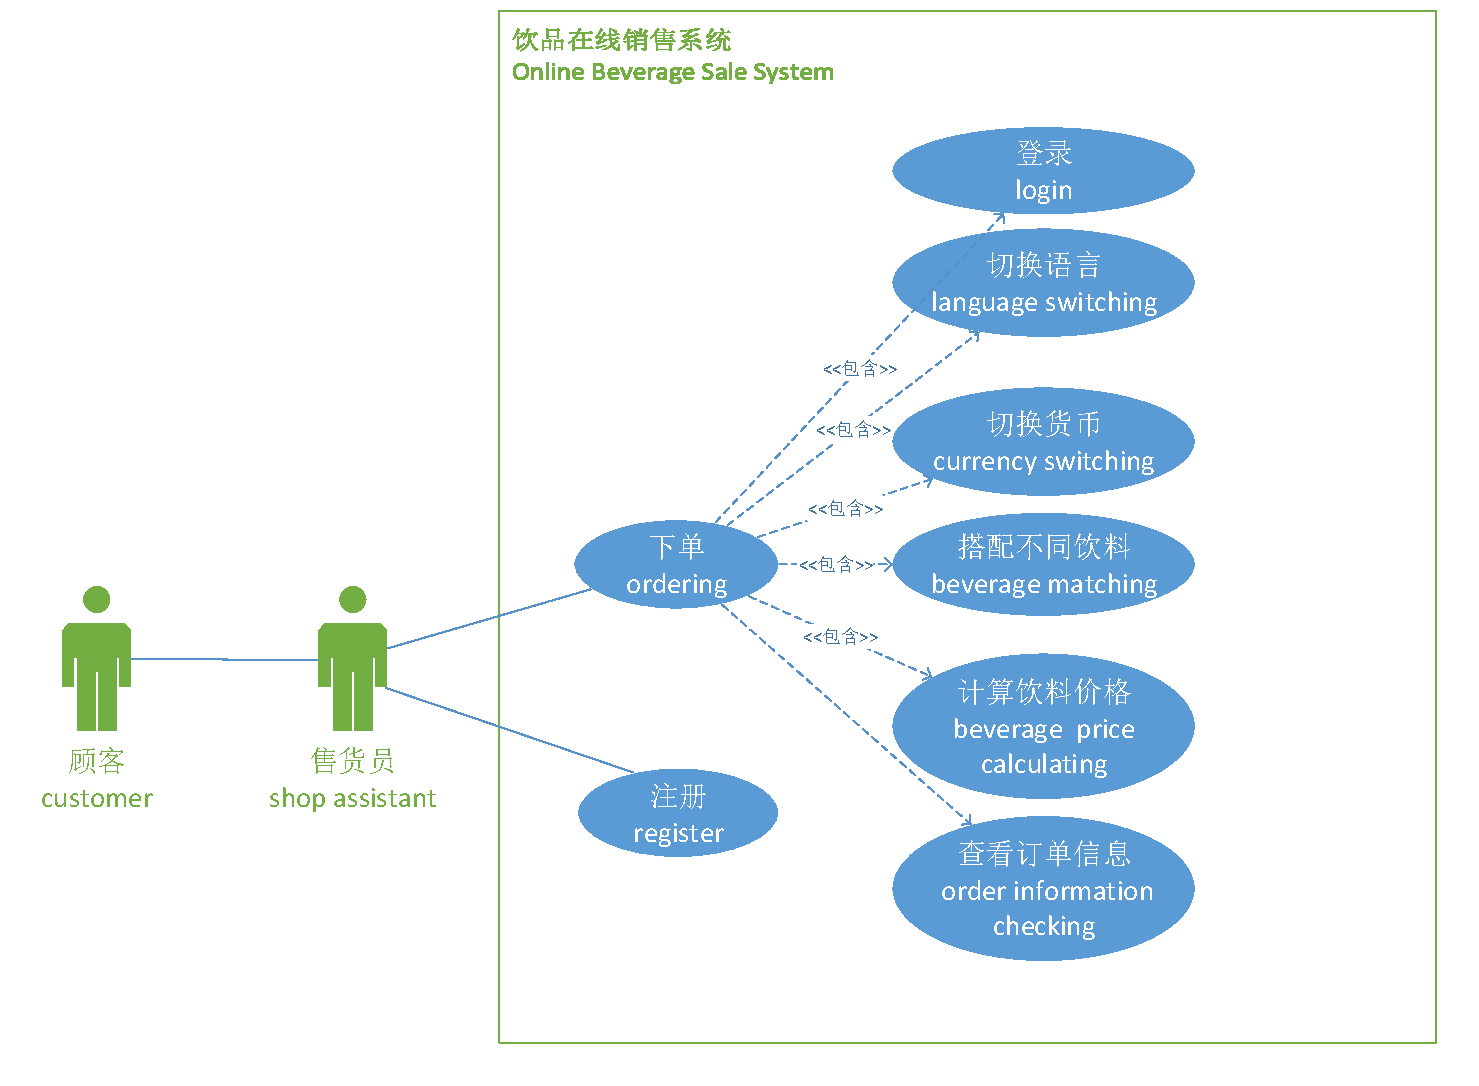
\includegraphics[scale=0.43]{useCase.pdf}
  \caption{Overall Use-case Diagram}\label{1}
\end{figure}

\subsubsection{Use case 1: Ordering}
In this use-case, we apply the swim lane diagram to concisely describe the relationship between users and the system.
\begin{figure}
  \centering
  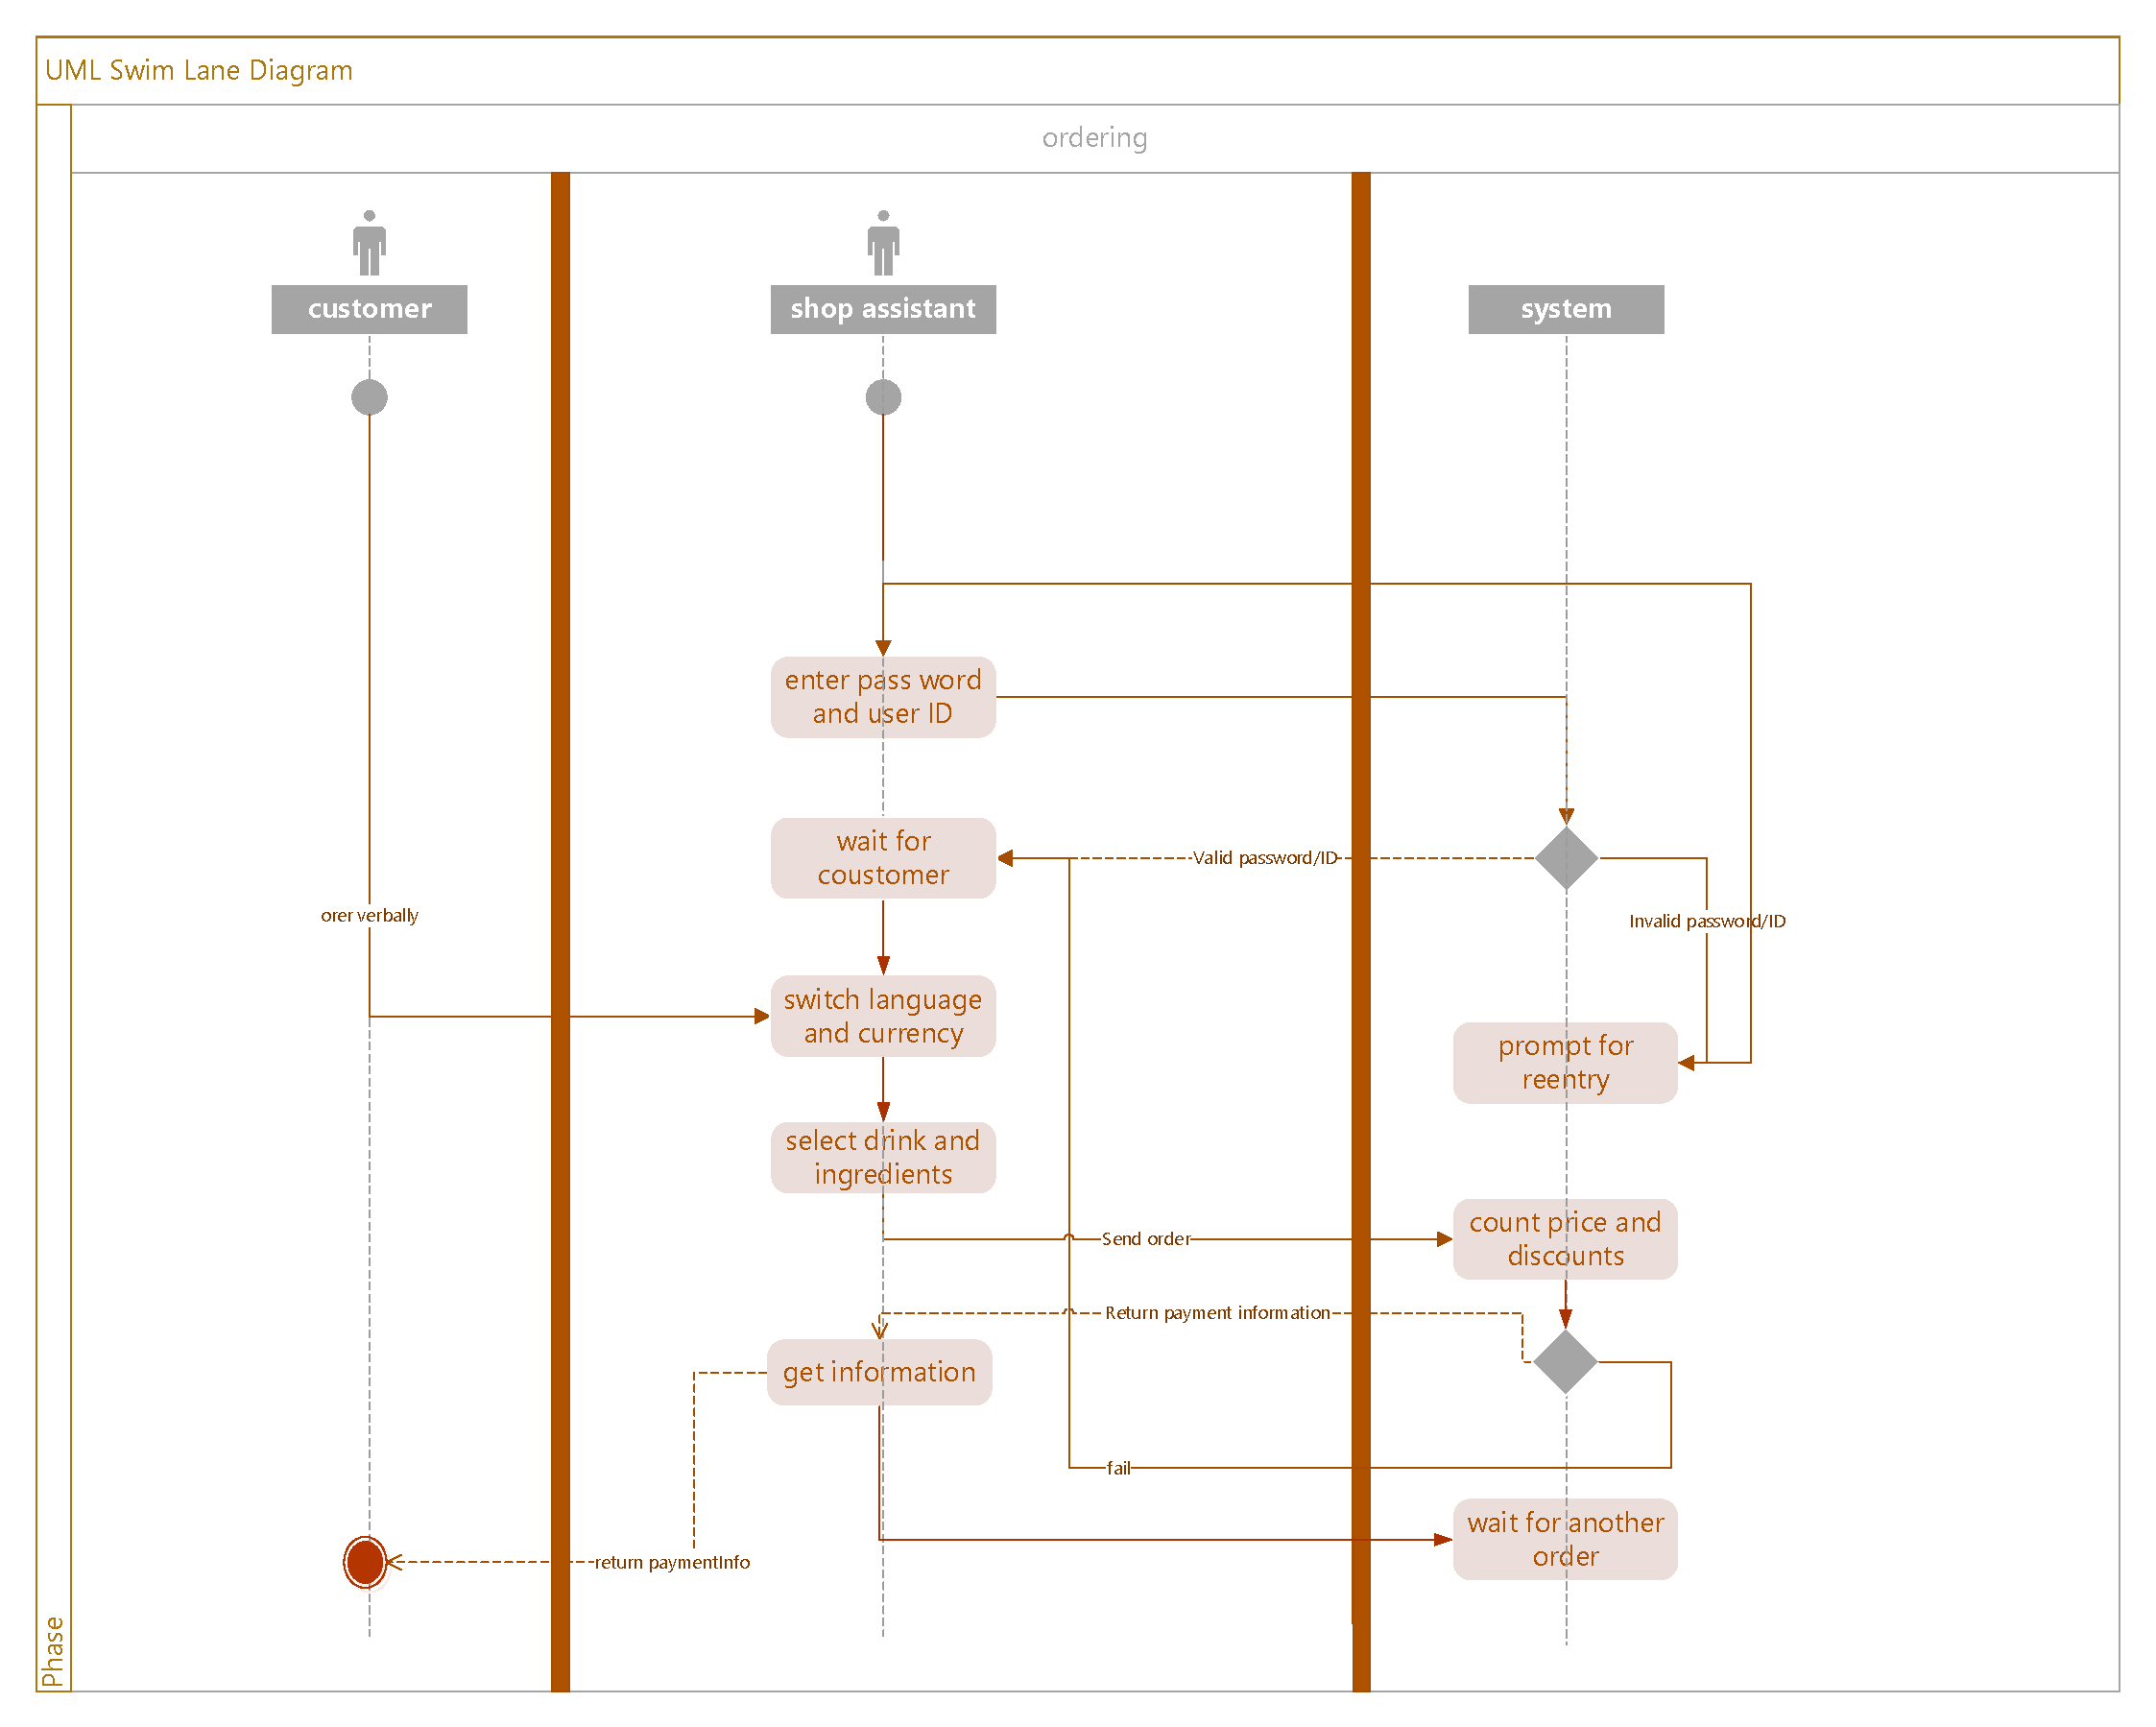
\includegraphics[scale=0.33]{SwimLane.pdf}
  \caption{UML Swim Lane Diagram}\label{2}
\end{figure}
\begin{itemize}
\item \textbf{Use-case name:} ordering
\item \textbf{Actors:} customers and shop assistants
\item \textbf{Target:} The shop assistant can complete the order-making process according to the verbal instruction of customers.
\item \textbf{Precondition:} The shop assistant has registered before. 
\item \textbf{Triggering condition:} There is a customer waiting to order in the store.
\item \textbf{Main scene:} After the shop assistant logs in the system successfully, he/she waits for the verbal instructions of the customer. After the customer tells him/her the wanted cup-size, ingredients and kind of  beverages, the shop assistant can make an ordering, and tells the customer the total price, discounted price and discount information of the order. After the customer has paid the charge, the order is finished and the system will be waiting for another order.
\item \textbf{Abnormal scenes:}
\begin{enumerate}
\item  \textbf{Login failure:} If the shop assistant enters wrong username or password, he can get the chance to enter again until he finally enters the correct username and password and logs in the system. 

\item \textbf{Order failure:} If the order process is interrupted due to the internet or other hardware break, the order process will restart a new order.\end{enumerate}
\item \textbf{Frequency:} The ordering use-case will be continuing 24 hours a day only if there is a customer waiting to order.
\end{itemize}

\subsubsection{Use case 2: Register}
In the ordering user-case, we apply the activity diagram to describe the whole process. 
\begin{figure}
  \centering
  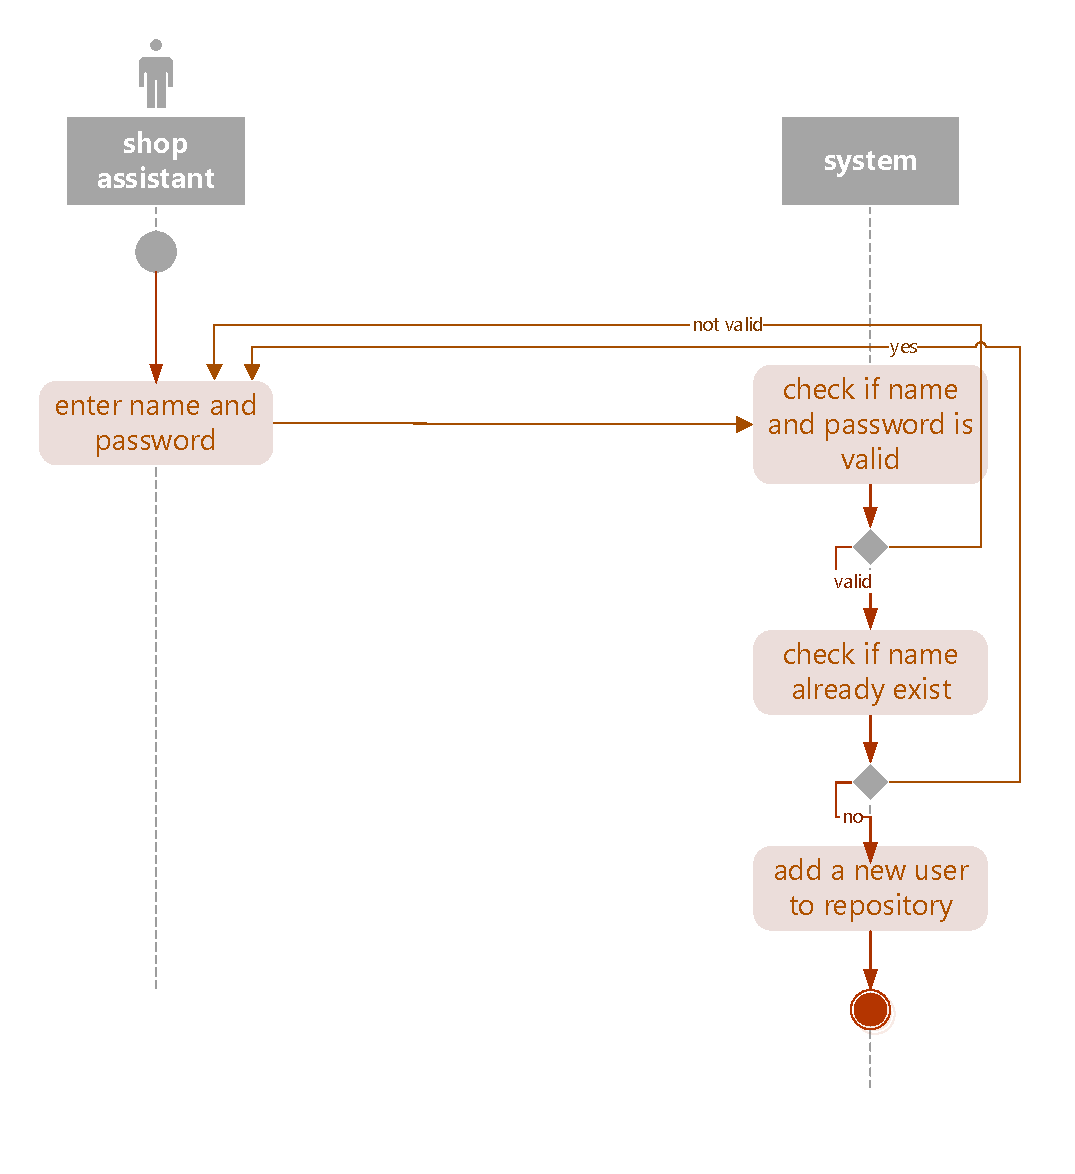
\includegraphics[scale=0.44]{ActivityDiagram.pdf}
  \caption{Overall Use-case Diagram}\label{3}
\end{figure}

 \begin{itemize}
\item \textbf{Use-case name:}  register
\item \textbf{Actors:} shop assistants
\item \textbf{Target:} The shop assistant can complete the register process.
\item \textbf{Precondition:} 
\begin{enumerate}
\item The server of the system is running normally.
\end{enumerate}
\item \textbf{Triggering condition:} None
\item \textbf{Main scene:} After the shop assistant gains the access authorization successfully, he can enter the system to choose login or register. After he enters the valid username and password, he can use them to login and make orders.
\item \textbf{Abnormal scenes:} 
\begin{enumerate}
\item  \textbf{Password invalid:} If the shop assistant enters invalid password, the system will prompt corresponding message and let the user enter again untill he enters the valid password.
\item \textbf{Username invalid:} If the shop assistant enters invalid username, the system will prompt corresponding message and let the user enter again until he enters the valid username.
\end{enumerate}
\item \textbf{Frequency:}  Relatively low, since only when there is new and unregistered shop assistant will it be triggered. However, the register use-case should be available 24 hours a day. 
\end{itemize}

\subsection{Class analysis and modeling}
\subsubsection{Analysis class extraction}
\begin{itemize}
\item User
\item AccountService
\item OrderItem
\item Order
\item PaymentInfo
\item OrderService
\item MarketingStrategy
\item DoubleElevenStrategy
\item FullDiscountStrategy
\item CombinationDiscountStrategy
\item LanguageService
\item MenuService
\end{itemize}

\subsubsection{Function of classes}
\begin{itemize}
\item \textbf{User :} The entity class represents shop assistants. There are two attributes: name and password.
\item \textbf{AccountService :} The service class is charge of the login, signup, status-checking, name-checking and password-checking of users.
\item \textbf{OrderItem :} The entity class represents beverages. There are three attributes: name, size and ingredients. Also, it has a public method to calculate the price according to its size and ingredients.
\item \textbf{Order :} The DTO class is used to transfer data from server to client end. There are three attributes: id, currency and orderItems. Also, it has a public method to calculate the total charge of the order. 
\item \textbf{PaymentInfo :} The class is composed of all the return information of the order, including price, discount, discountPrice and messages.
\item \textbf{OrderService :} The service class includes one attribute strategies and one public method pay.
\item \textbf{MarketingStrategy :} The strategy class include one public method getDiscount. And all the  sub strategy classes including  DoubleElevenStrategy, FullDiscountStrategy and CombinationDiscountStrategy inherit it.
\item \textbf{LanguageService :} The service class has one public method updateLanguage.
\item \textbf{MenuService :} The service class has one public method getPrice according to different countries and regions.
\end{itemize}
\subsubsection{Relationship between classes}
As the UML diagram shows, the relationships in this system can be divided into three kinds: inheritance, composition and dependency.
\begin{figure}
  \centering
  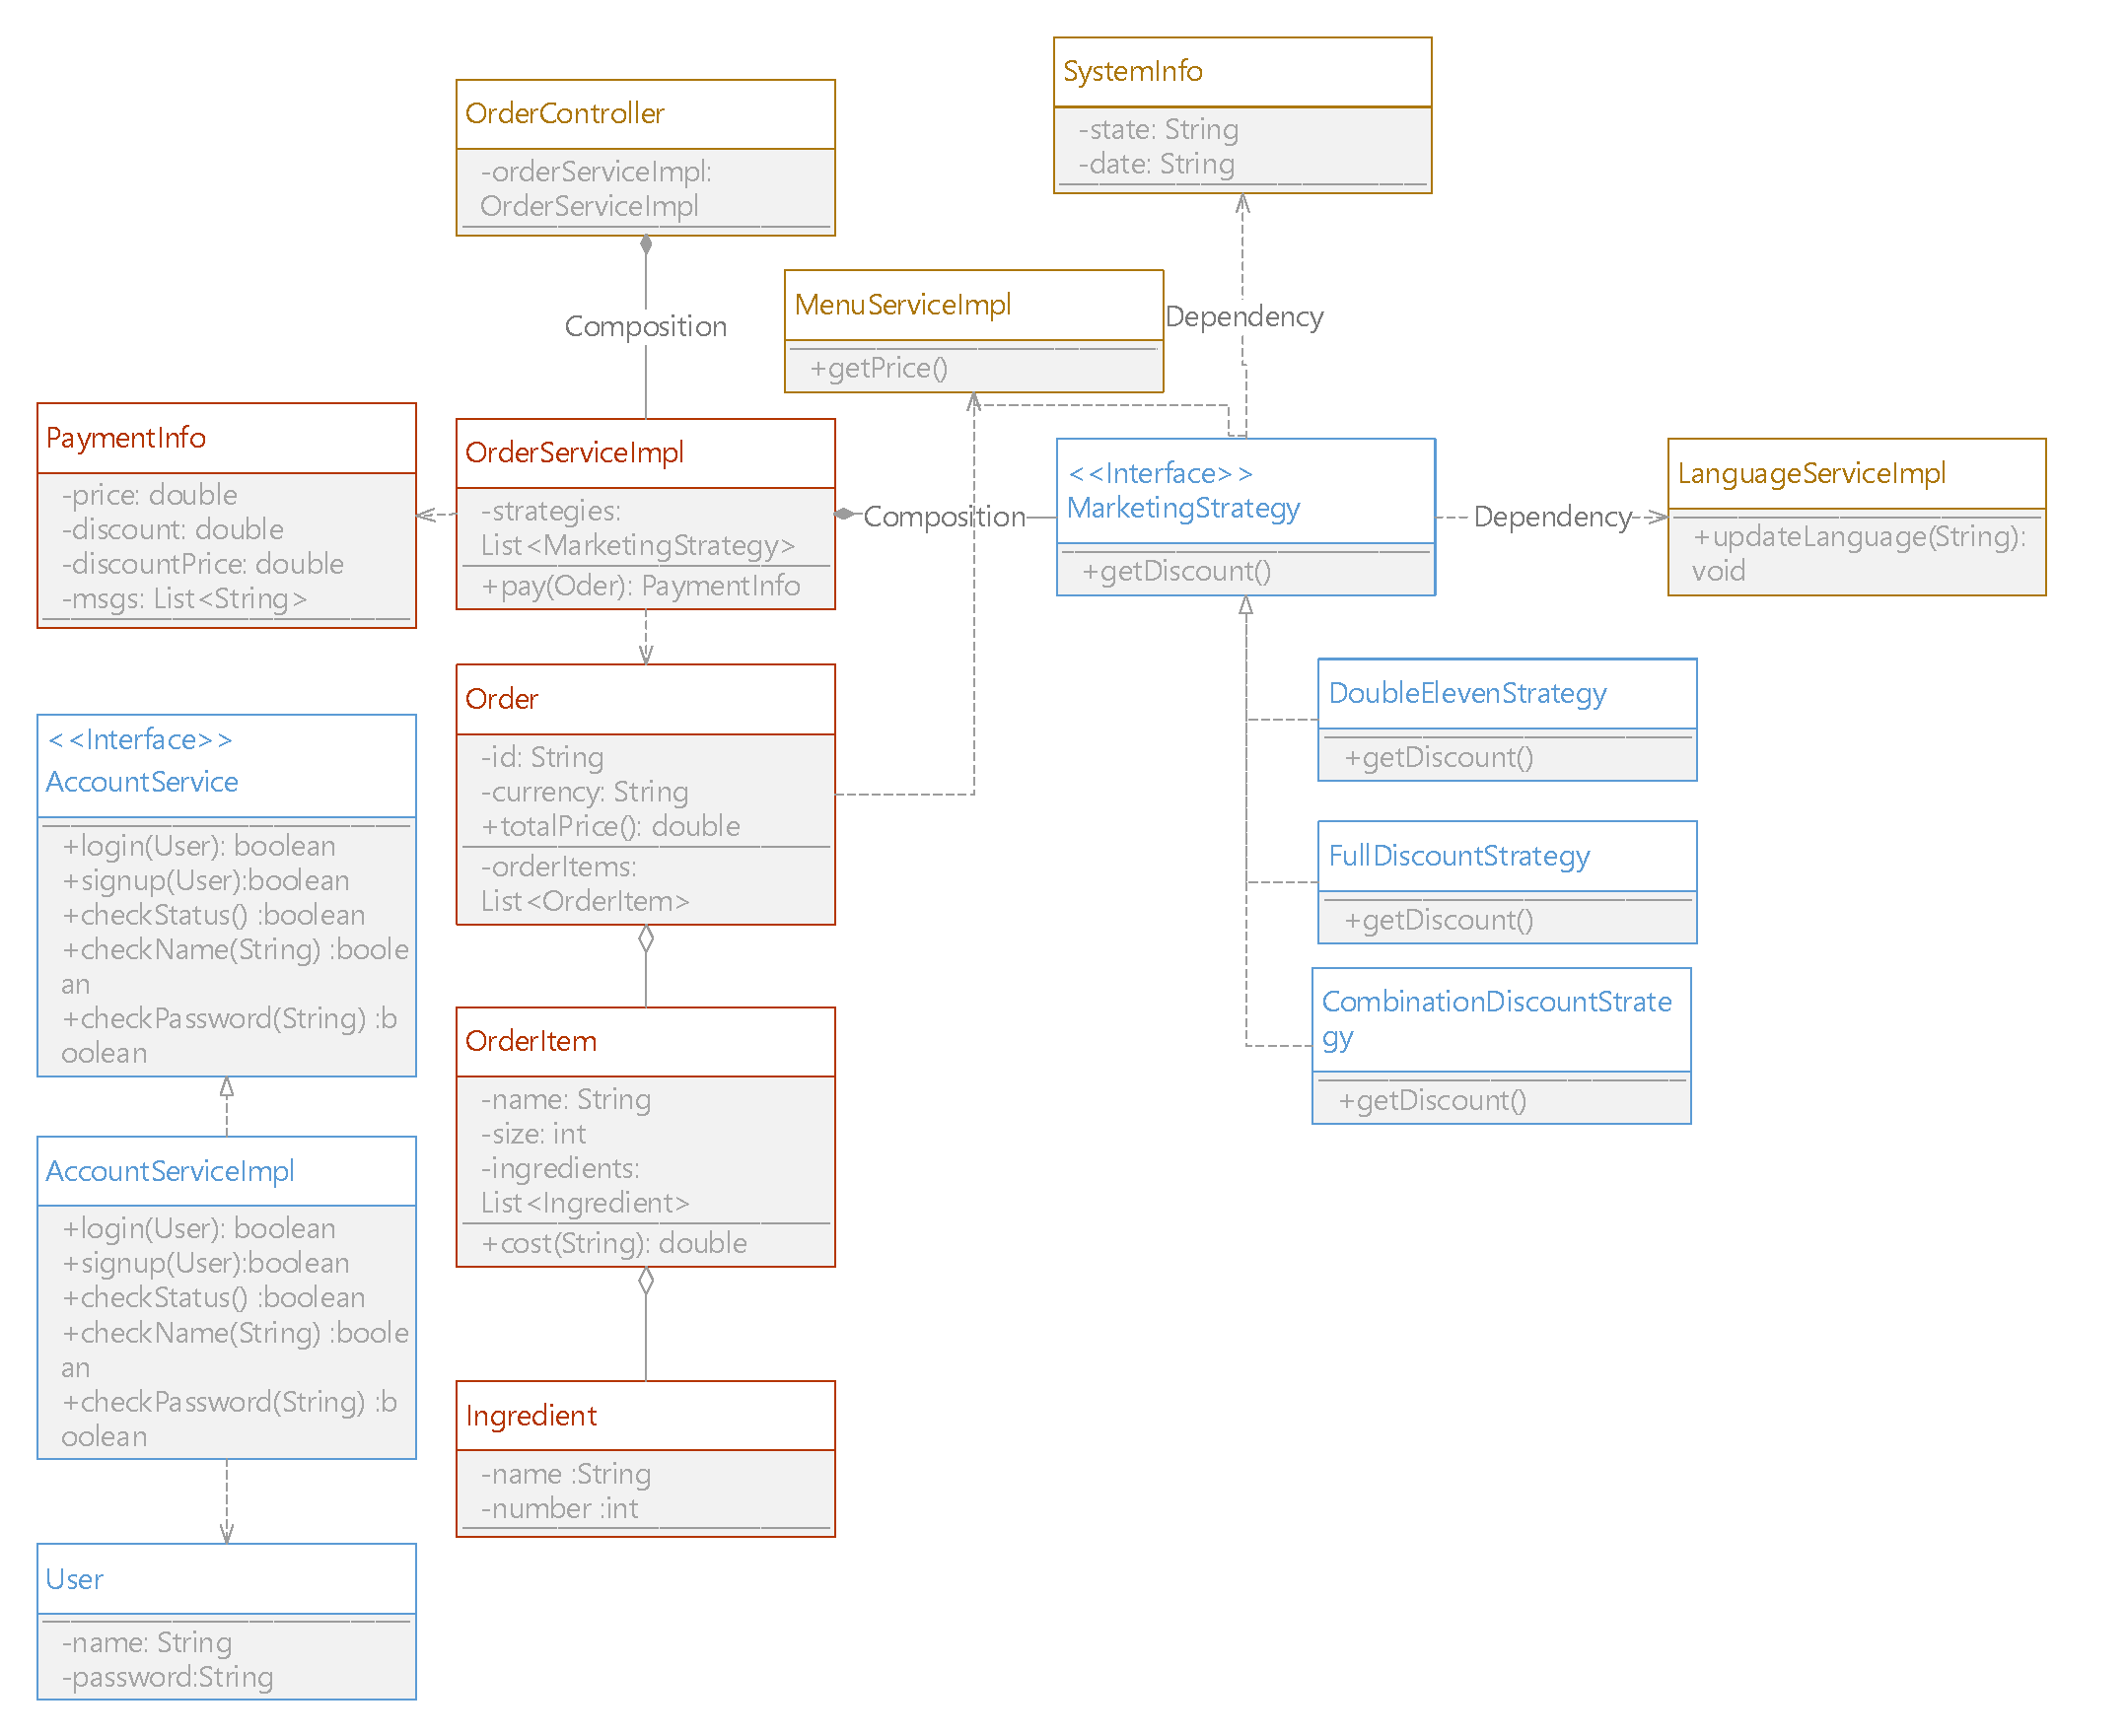
\includegraphics[scale=0.38]{UMLClass.pdf}
  \caption{Overall UML Class Diagram}\label{4}
\end{figure}
\subsection{Data Flow analysis and modeling}
We apply the DFD(data flow diagram) to describe the flow of the input data and output data.
We 
\subsubsection{level 0:} The top/level-0 diagram is an overall description of the whole system. The external entity are only control panel and control panel display. The data flow diagram for level 0 is shown as Figure \ref{5}. We can see what our system does is to process the order information and produce the corresponding payment information.
\begin{figure}
  \centering
  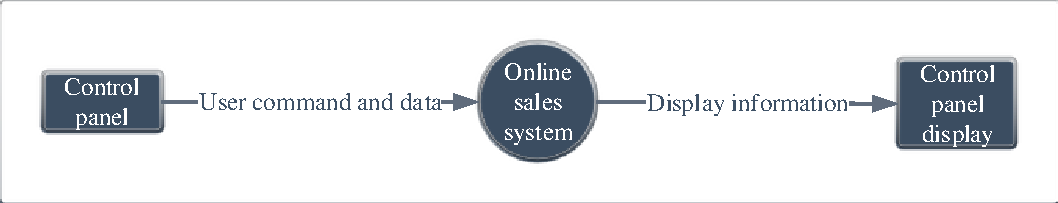
\includegraphics[scale=0.38]{DataFlowLevel0.pdf}
  \caption{Data Flow Level 0 Diagram}\label{5}
\end{figure}
\subsubsection{level 1:}
We can see a more detailed description of the whole process from the level-1 diagram in Figure \ref{6}. The order information flows from price-counting, sales-plan choosing and finally changes into payment information and shows in the control panel display.
\begin{figure}
  \centering
  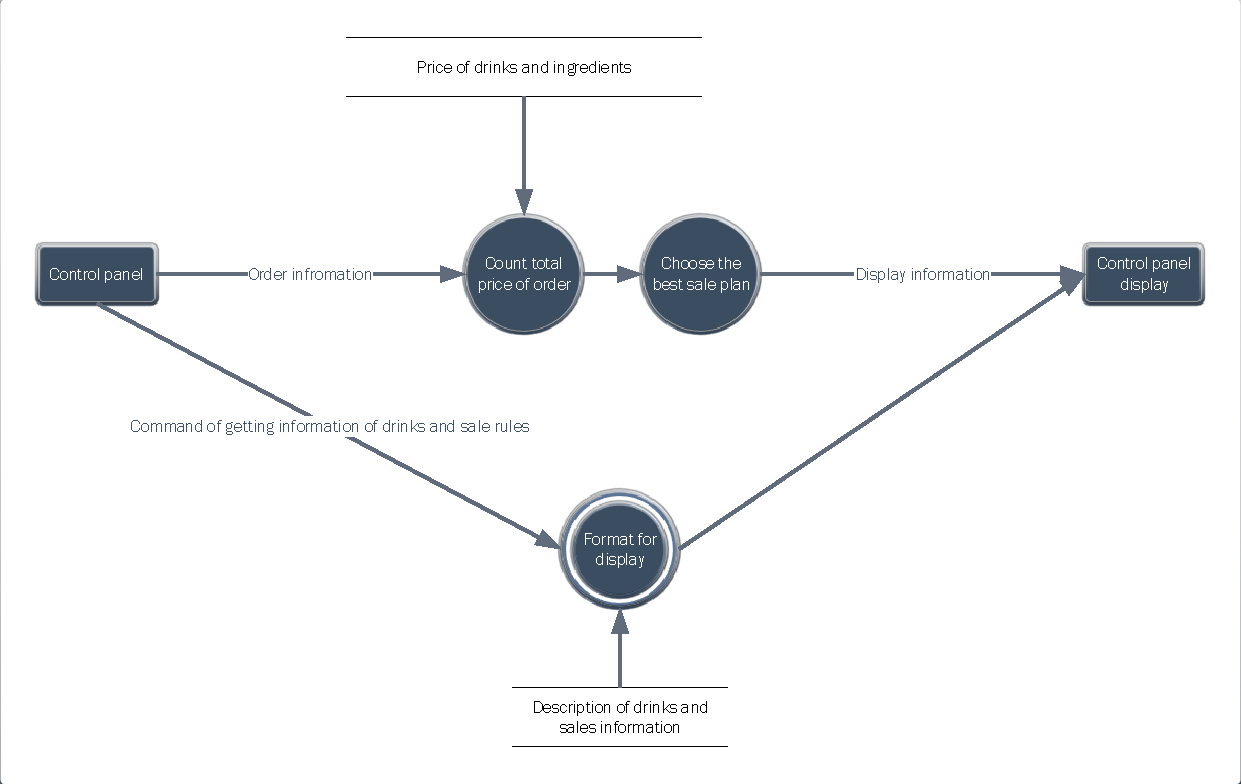
\includegraphics[scale=0.38]{DataFlowLevel1.pdf}
  \caption{Data Flow Level 1 Diagram}\label{6}
\end{figure}

\subsection{Behavior analysis and modeling}
In this part, we apply the UML status diagram to conduct the behavior analysis and modeling.
\subsubsection{Whole status transfer}
We can see from the Figure \ref{7} that the status of the system can be divided into three parts: waiting for login/register, waiting for ordering and ordered. And the system will be continuing waiting until it is activated with order information. It processes the order, returnes the payment information and continues its waiting.
\begin{figure}
  \centering
  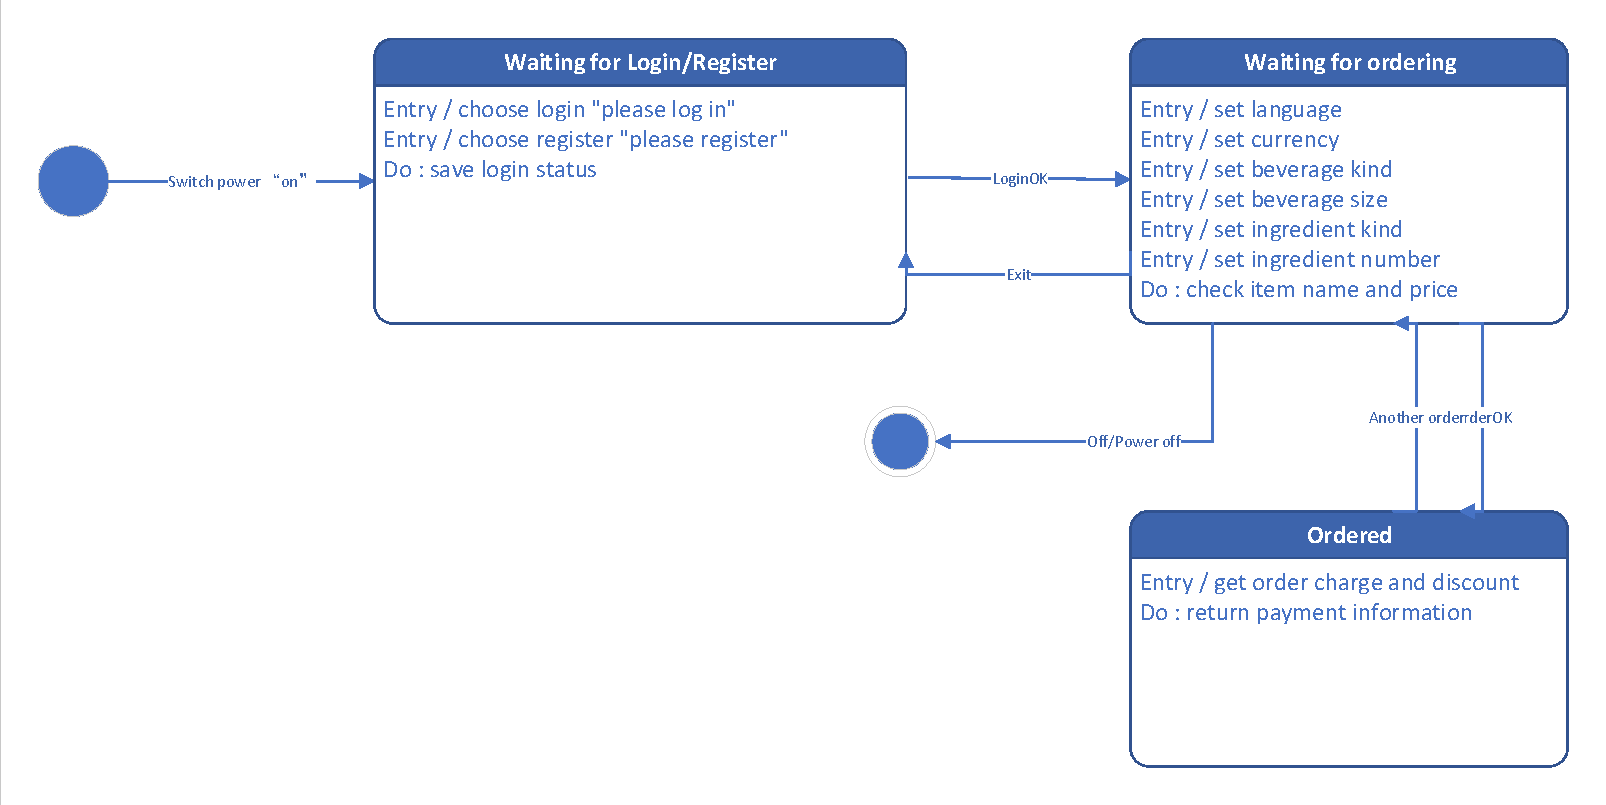
\includegraphics[scale=0.38]{statusDiagram.pdf}
  \caption{UML Status Diagram}\label{7}
\end{figure}
% Huang 2019-06-23 above
\chapter{Performance Demands}

\section{Massive end user support}
\subsection{Detailed Description}
There will be about 200 stores using this system at the same time. And the sale scale will be about 1000 people per day. The people using this system includes customers and shop assistants.
\subsection{Proposed measures}
Since the system will be built on several servers, the strategies like load balancing can be used to handle the big amount of customers.

\section{Stability over long period of time}
\subsection{Detailed Description}
Since the store will be open 24 hours a day, the system must be running all the time and at least maintained evert half a year. Also, the response time of every order  should be less than 2 seconds.
\subsection{Proposed measures}
This requires that the system should not stop or exit by accident at any time. We should handle all the possible accidents and catch the exceptions. And we should try every means to enhance the speed of the system.

\chapter{Appendix}
\section{Demand interview outline}
\subsection{Constraints (5 minutes)}
\begin{enumerate}
\item What is the number of servers? 
\item Is there a regulation or limitation on the system running server-side operating system? 
\item What are the rules or restrictions for the client device operating system (in the store)? 
\item Is the salesperson's computer equipped with a screen for the customers?
\item Are there still any other special hardware conditions (supplementary)? 
\item Does the company have specific legal restrictions? 
\item The development time and delivery time points given? 
\item Is there an intermediate time frame when partial project need to be examined?
\end{enumerate}
 \subsection{Performance requirements (5 minutes)}
 \begin{enumerate}
\item Is 1,000 person/day referring to the salesperson or the customer (personal * month) ? What is the upper limit? 
\item What is the number of the stores in the description ``Support the usage of massive stores concurrently''?  What is the average number of orders in the store? And what about the peak order number? 
\item Order response time? 
\item ``Long-running and stable support system ": the requirements for a client front end and user-friendliness, cannot be unable to play due to any reason except network or hardware issues, cannot crash under massive clients, cannot have severe bug after online
\end{enumerate}
\subsection{Functional requirements(15 minutes)}
\begin{enumerate}
\item Drinks, ingredients, cups in the beverage store supported by the system 
\item Superposition and mutual exclusion of offers 
\item Language, currency, pricing 
\item Register \& log in 
\item Order versus Associate / independent with drinks, price, and description?
\item What the customer sees: the information returned in the order content and paymentInfo , including the beverage, original price, discounted price, discount information (whether it is necessary to specify the description of each beverage) 
\item How the salesperson gets permission 
\item Log information provided by the system 
\item Process confirmation again
\end{enumerate}
\subsection{Possible modification of the code}
\begin{enumerate}
\item Increase currency dollar 
\item Salesperson access 
\item Offer modification 
\item View all aspects of drinks and ingredients (cup type, price) individual customer / salesperson interface 
\end{enumerate}
\subsection{About the requirements document }
\begin{enumerate}
\item ``Give a corresponding map and explanation for each demand"
\end{enumerate}
\section{Organized interview records}
\subsection{Constraints (5 minutes)}
\begin{enumerate}
\item What is the number of servers? 
\par
There are 200 stores belonging to the company, each will treat 1000 customers each day. 
\par
The 1000 customers is a approximate number. It is a non-functional restriction and this might influence another function - the order number, which should be unique considering the order number stated below.
\item Is there a regulation or limitation on the system running server-side operating system? 
\par
The infrastructure of the system has no restriction and should be purchased. We should consider the budget while considering the hardware specifications.
\item What are the rules or restrictions for the client device operating system (in the store)? 
\par
The infrastructure of the system has no restriction and should be purchased. We should consider the budget while considering the hardware specifications.
\item Is the salesperson's computer equipped with a screen for the customers?
\par
Yes.
\item Are there still any other special hardware conditions (supplementary)? 
\par
No.
\item Does the company have specific legal restrictions? 
\par
The salesperson should not have access to the modification of the price of the drinks.
\item The development time and delivery time points given? 
\par
The project should be finished in 2 months.
\item Is there an intermediate time frame when partial project need to be examined?
\par
No.
\end{enumerate}
 \subsection{Performance requirements (5 minutes)}
 \begin{enumerate}
\item Is 1,000 person/day referring to the salesperson or the customer (personal * month) ? What is the upper limit? 
\par
The 1000 customers is a approximate number. It is a non-functional restriction and this might influence another function - the order number, which should be unique considering the order number stated below.
\par
The upper limit will not be too greater than the general expectation above.
\item What is the number of the stores in the description ``Support the usage of massive stores concurrently''?  What is the average number of orders in the store? And what about the peak order number? 
\par
The system should support the service with the customer number stated above. The average number is the customer number stated above and the peak number will not be too much greater than the average number.
\item Order response time? 
\par 
The response time is 2 seconds for each order. It means from the order successfully created in the front end to the result of the order from the back end sent to the front end.
\item ``Long-running and stable support system ": the requirements for a client front end and user-friendliness, cannot be unable to play due to any reason except network or hardware issues, cannot crash under massive clients, cannot have severe bug after online
\par
The system should run 24 hours a day and should not break down because of the program rather than physical problems. If an order is interrupted because of the network issues, the system can simply discard the order information.
\end{enumerate}
\subsection{Functional requirements(15 minutes)}
\begin{enumerate}
\item Drinks, ingredients, cups in the beverage store supported by the system 
\par
The drinks provided currently are coffee and tea, where coffee includes Cappuccino and Espresso and tea includes Red Tea and Green Tea. The ingredients includes chocolate and cream while the cup size vary from small cup, the middle cup to the large cup.
\item Superposition and mutual exclusion of offers 
\par
The first three offers and the last offers are superposition offers, while the full discount offer and the double eleven offer are different.
\item Language, currency, pricing 
\par
The price is different for each currency and we need to provide a price table for each of the currency we provide. In the meanwhile, we still need to provide a description for each item on the menu in each language we provide. That is to say, the menu should have versions according to the languages.
\par
These information are available after the order in the system. The order placing operation includes generating these information.
\par
In addition, the US Dollar is added into the system while the languages provided remain the same.
\item Register \& log in 
\par
The detailed specification for the register and log in function are the same as Lab 3, and the requirement documentation for Lab 3 can be referred.
\item Order versus Associate / independent with drinks, price, and description?
\item What the customer sees: the information returned in the order content and paymentInfo , including the beverage, original price, discounted price, discount information (whether it is necessary to specify the description of each beverage) 
\par
The customer can place order via the staff and what the customer interact with the system is not considered.
\item How the salesperson gets permission 
\par
A valid log in operation should enable the salesperson with permission.
\item Log information provided by the system 
\par
The log information have two parts. There is an error log and a info log. When there is an error when placing the order, the order number should be recorded in the log whereas the order number is neglected when the error is not generated in the process of placing an order. 
\par
The language of the log should be English and it should be independent of the language switch of the application.
\item Process confirmation again
\par
The process of the order is confirmed and remain the same as the previous lab requirements.
\end{enumerate}
\subsection{Possible modification of the code}
\begin{enumerate}
\item Add the US Dollar currency 
\item Restrict the salesperson access 
\item Offer modification 
\item View all aspects of drinks and ingredients (cup type, price) individual customer / salesperson interface 
\end{enumerate}
\subsection{About the requirements document }
\begin{enumerate}
\item ``Give a corresponding map and explanation for each demand"
\end{enumerate}
\section{Code change logs in response of new demands}
\subsection{Aspects for code change}
\begin{enumerate}
\item \textbf{Currency change: } According to the requirement revision, we add the USD currency menu and corresponding order tests.
\item \textbf{Login change: } To enhance the user-friendliness, we dispatch the runtime exception of login failure, record the possible errors in log files and provide the reentry chance for users.
\item \textbf{Log information files: } For consistency, we record all the log information related to ordering in the log files (error.log and trace.log under the logs directory) through the function of Logger.
\item \textbf{Sales strategy change: } We change the level and kind of the sales strategies according to the requirement alternation, and add the relative tests.
\end{enumerate}
\subsection{Revision history of the code}
\begin{tabular}{|c|c|c|l|}
\hline 
Modifier&Modify Time&Approver&Commit Message\\
\hline  
Huang, Jiani&Jun 14, 2019&All&feat add the tea and coffee discount to combinationDiscount Strategy\\
\hline
Huang, Jiani&Jun 14, 2019&All&feat change the test file for combination discount strategy
\hline
Huang, Jiani&Jun 14, 2019&All&feat add the country America
\hline
Huang, Jiani&Jun 14, 2019&All&feat feat #2625717 revise the usd menu for the two new drinks
\hline
Liu, Jiaxing&Jun 23, 2019&All&feat add two log files and correct the double eleven strategy
\end{tabular}


\begin{thebibliography}{A}
\bibitem{1}
Wikipedia contributors. (2019, March 22). JUnit. In \emph{Wikipedia, The Free Encyclopedia}. Retrieved 14:53, April 1, 2019, from \url{https://en.wikipedia.org/w/index.php?title=JUnit&oldid=888928403}
\end{thebibliography}
\end{document} 